\section{Introduction}
We will implement an algorithm to solve any Sudoku puzzle, if it has a solution. Sudoku is puzzle consisting of $9*9$ squares split into 9 $3*3$ fields. Each square can hold a number between $1-9$. A valid solution to the puzzle ensures that each number only appears once in every column, once in every row and once in every $3*3$ field. Figure 1 shows a valid solution to a Sudoku puzzle. 
\begin{figure}[h]
\centering
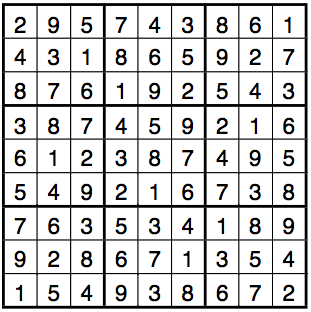
\includegraphics[width=9cm]{Sudoku.png}
\caption{A valid solution to a Sudoku puzzle.}
\end{figure}

\noindent The algorithm we will implement is a forward-checking algorithm based on arc consistency. The GUI allows a user to enter an initial assignment of variables and then press the button \textit{solve} to start the solving algorithm.

\section{Setup}
To set up the algorithm we initialize a \texttt{ArrayList<ArrayList<Integer>>} of size 81 that we call \texttt{D}. The outer array represents the squares in the Sudoku puzzle and the inner array is the remaining valid domain of each square. Initially all the inner arrays contain the values $1-9$. 

\section{Forward checking}
The forward checking algorithm \texttt{FC} takes an \texttt{ArrayList<Integer>} as input. It is the assignment of the squares. The algorithm finds the index of the first unassigned variable by searching for the index of the first variable in the array that is $0$, as we use $0$ to represent unassigned variables. If no unassigned variables exist the algorithm return the given assignment without modification, as it must be a valid solution. The algorithm finds the unassigned variables possible assignments by looking its domain up in \texttt{D}. It then go through the variables in the domain one by one, checking if an assignment is arc consistent by calling the method \texttt{AC\_FC}. If the assignment is not arc consistent the algorithm tries another variable in the domain.

If on the other hand the assignment is arc consistent the algorithm recursively finds the next unassigned square and repeats the process until there are no more unassigned variables. If no valid assignment is found the method returns \texttt{null}. Backups of both \texttt{D} and the domain of the current square are created in case we need to backtrack because some assignment was not arc consistent.

\section{Solve}
The method \texttt{solve} is called if the button \textit{solve} is pressed. The method first checks if the initial assignment of variables is arc consistent \texttt{FC} is called with the initial assignment. The method returns true if \texttt{FC} return a non \texttt{null} value.

\section{Conclusion}
The algorithm works as intended, and we have not spotted any mistakes in the returned assignments. The algorithm is fast if very few or very many variables are set initially. This is because there are generally several valid solutions to puzzles with very few initial assignments and thus enforcing arc consistency generally does not result in backtracking. If very many initial variables are set the domains are so small that there are few possible assignments to check. The allegedly hardest Sudoku puzzle\footnote{http://www.conceptispuzzles.com/picture/12/4154.png} takes around 50 seconds to solve using our algorithm.